\documentclass[11pt]{article}
\usepackage[utf8]{inputenc}	% Para caracteres en español
\usepackage{amsmath,amsthm,amsfonts,amssymb,amscd}
\usepackage{multirow,booktabs}
\usepackage[table]{xcolor}
\usepackage{fullpage}
\usepackage{lastpage}
\usepackage{enumitem}
\usepackage{fancyhdr}
\usepackage{mathrsfs}
\usepackage{wrapfig}
\usepackage{setspace}
\usepackage{calc}
\usepackage{multicol}
\usepackage{cancel}
%\usepackage[retainorgcmds]{IEEEtrantools}
\usepackage[margin=3cm]{geometry}
\usepackage{amsmath}
\newlength{\tabcont}
\setlength{\parindent}{0.0in}
\setlength{\parskip}{0.05in}
\usepackage{empheq}
\usepackage{framed}
\usepackage[most]{tcolorbox}
\usepackage{xcolor}
\colorlet{shadecolor}{orange!15}
\parindent 0in
\parskip 12pt
\geometry{margin=1in, headsep=0.25in}
\theoremstyle{definition}
\newtheorem{defn}{Definition}
\newtheorem{reg}{Rule}
\newtheorem{exer}{Exercise}
\newtheorem{note}{Note}

%my additions
\usepackage{graphicx}
\usepackage{caption}
\usepackage{tikz}
\usetikzlibrary{bayesnet}

%for figure referencing in-text
\usepackage[hidelinks]{hyperref}
\usepackage{cleveref}
%for biliography
%\usepackage[backend=bibtex,style=authoryear-comp,natbib=true]{biblatex}
%\addbibresource{luis.bib} % The filename of the bibliography

%for drawing boxes around text
\usepackage[linewidth=1pt]{mdframed}

%for under- and overbrace
\usepackage{mathtools}

%appendix management
\usepackage[toc,page]{appendix}

\begin{document}

\thispagestyle{empty}

%------------------------------
%	HEADLINE
%------------------------------
\begin{center}
{\LARGE \bf Concept Notes: Transformer architecture}\\
{\large Luis Oala}\\
\today
\end{center}

%------------------------------
%	DOCUMENT
%------------------------------
\begin{center}
	{\Large \bf Materials used}
	\\
	These notes are based on the following materials
\end{center}
\begin{itemize}
	\item ...
\end{itemize}

Attention is a popular computational module in many successful neural language models but also finds application in vision tasks such as visual question answering. The purpose of this short concept note is to concisely explain the mechanics of a model architecture called Transformer which solely uses attention. This note solely focuses on the mechanics of the Transformer model. The goal is to make clear what computations are actually carried out and how the model works. I do not discuss the conceptual merits of attention per se or why it is useful for sequence modelling tasks.
\par The notes start with a short exposition of attention as 'classically' used in neural sequence-to-sequence models based on LSTM cells. Then the Transformer's main mechanism, as introduced by \cite{vaswani_attention_2017}, is explained in detail. Finally, a short mention is made of the Universal Transformer idea by \cite{dehghani_universal_2018}, who address a practical and theoretical shortcoming of the original architecture.
\section{Attention as we know it}

\begin{figure}[h]
	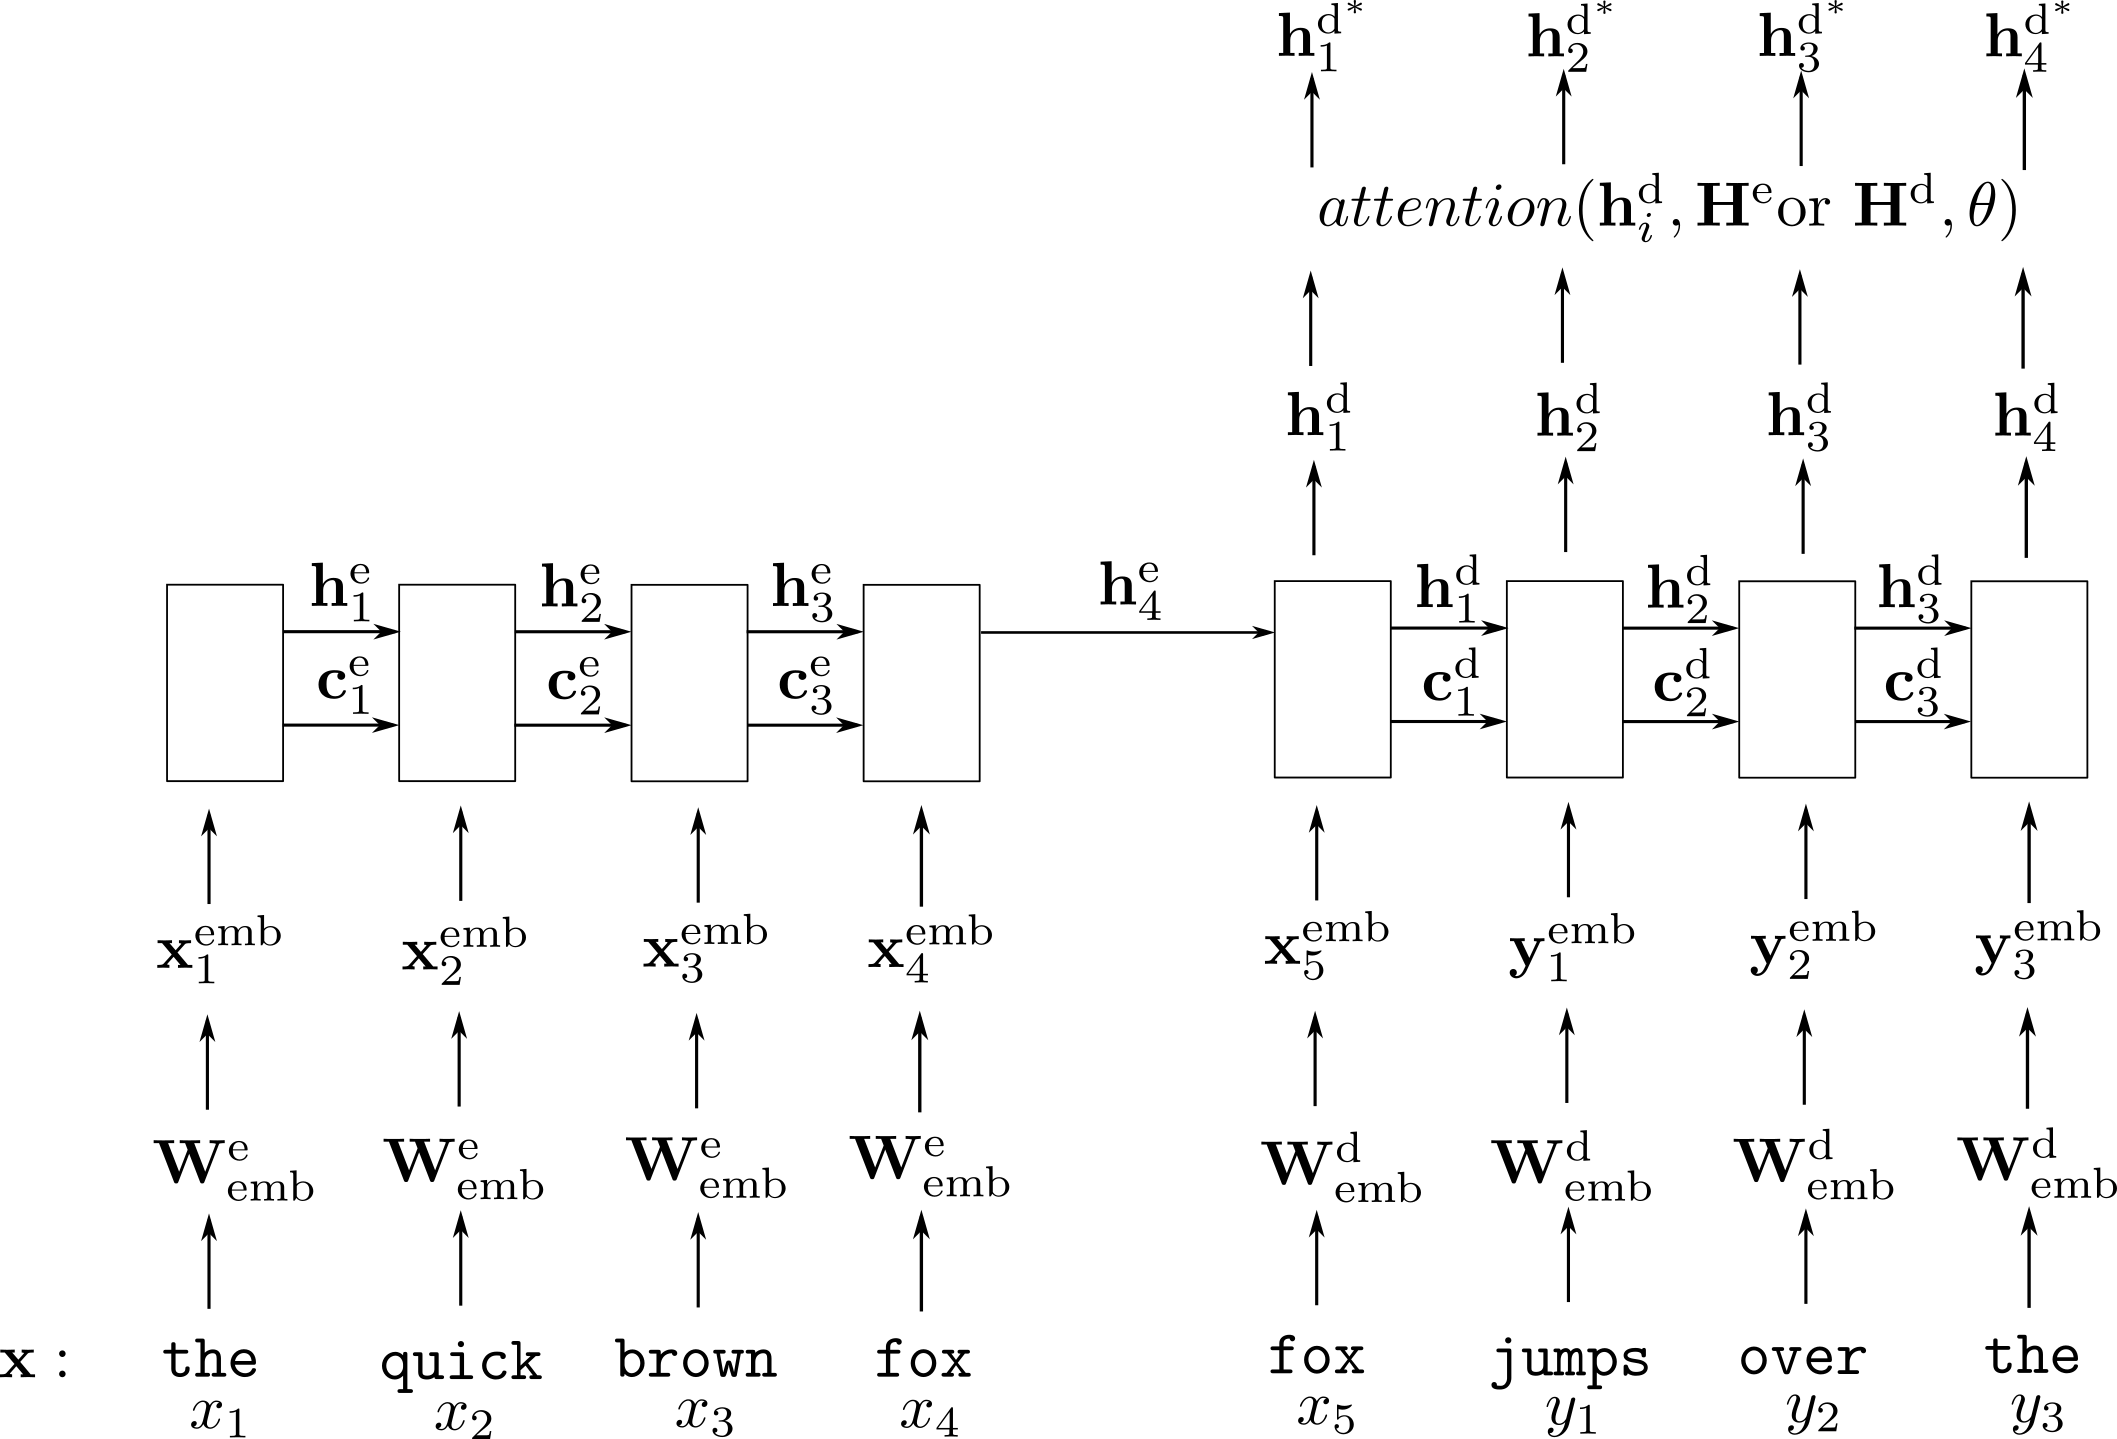
\includegraphics[width=\linewidth]{figures/vanilla-attention-big.png}
	\caption{Illustrated example of a vanilla encoder-decoder sequence-to-sequence architecture with an attention mechanism. The ouput mechanics of the decoder after $\mathbf{h}^{\text{d}^*}_i$ are omitted for brevity.}
	\label{fig:vanilla-attn}
\end{figure}

\autoref{fig:vanilla-attn} shows the sketch of a vanilla neural sequence-to-sequence model based on LSTM cells which utilizes an attention mechanism before the ouput layer of the decoder. We can make note of the following variables:
\begin{itemize}
	\item $\mathbf{h}^{\text{e}}_i$: the hidden state of the encoder LSTM cell at input sequence position $i$
	\item $\mathbf{h}^{\text{d}}_i$: the hidden state of the decoder LSTM cell at output sequence position $i$
	\item $\mathbf{H}^{\text{e}} = concat(\mathbf{h}^{\text{e}}_1,\dots ,\mathbf{h}^{\text{e}}_k)$: a matrix of all the hidden states of the encoder LSTM cell
	\item $\mathbf{H}^{\text{d}} = concat(\mathbf{h}^{\text{d}}_1,\dots ,\mathbf{h}^{\text{d}}_l)$: a matrix of all the hidden states of the decoder LSTM cell
	\item $\theta$: the trainable parameters of the attention function, varies depending on the design of the attention function
	\item $\mathbf{h}^{\text{d}^*}_i$: the decoder attention state at output sequence position $i$
\end{itemize}
The attention function then takes as input the current hidden state of the decoder $\mathbf{h}^{\text{d}}_i$, in the attention context also called \textit{query}, as well as a matrix $\mathbf{H}$ of other states for which we desire to calculate the attention distribution. $\mathbf{H}$ is also referred to as \textit{key} and \textit{value}. The parameters $\theta$ are the final inputs to the attention function. These parameters are learned to train the model's attention mechanism.
\par
The attention function $attention(\mathbf{h}^{\text{d}}_i, \mathbf{H}^{\text{e}} \text{or } \mathbf{H}^{\text{d}}, \mathbf{\theta})$ usually contains the following steps and components:
\begin{itemize}
	\item[(a)] Calculate \textit{attention scores} $\mathbf{e}_i$,
	\item[(b)] normalize the \textit{attention scores} to an \textit{attention distribution} $\mathbf{a}_i$ via the softmax function
	\item[(c)] and finally combine the attention values, $\mathbf{H}$, into an attention weighted representation $\mathbf{h}^{\text{d}^*}_i$ using $\mathbf{a}_i$ as weights.
\end{itemize}
Let us look at a concrete example for these steps taken from \cite{see_get_2017}. In step (a) $\mathbf{e}_i$ is calculated as
\begin{equation}
	\mathbf{e}_i = \mathbf{v}^T\tanh(\mathbf{W}_1\mathbf{H} + \mathbf{W}_2 \mathbf{h}^{\text{d}}_i + \mathbf{b}_{\text{attn}})
	\label{eq:scores}
\end{equation}
Note that $i$ indicates the decoder time step in this context and for this particular kind of attention function we have $\theta = (\mathbf{W}_1,  \mathbf{W}_2, \mathbf{b}_{\text{attn}}, \mathbf{v})$. Thus we now have a vector $\mathbf{e}_i$ of \textit{attention scores}. Each position in $\mathbf{e}_i$ corresponds to a time step of the encoder LSTM cell. Next for step (b) these values are normalized via the softmax function to yield an \textit{attention distribution}:
\begin{equation}
	\mathbf{a}_i = \text{softmax}(\mathbf{e}_i)
	\label{eq:dist}
\end{equation}
Finally, in step (c) the attention scores are used to produce the \textit{context vector} $\mathbf{h}^{\text{d}^*}_i$:
\begin{equation}
	\mathbf{h}^{\text{d}^*}_i = \mathbf{H}\mathbf{a}_i
	\label{eq:context}
\end{equation}
Now we have worked through a concrete example for an attention function $attention(\mathbf{h}^{\text{d}}_i, \mathbf{H}^{\text{e}} \text{or } \mathbf{H}^{\text{d}}, \mathbf{\theta})$. Note that there many variants to design the attention function. Most variants only differ in the way $\mathbf{e}_i$ is calculated in \autoref{eq:scores}. The basic steps remain the same. 
\par 
After we have obtained the \textit{context vector} $\mathbf{h}^{\text{d}^*}_i$ it is then usually concatenated to the regular decoder output state $\mathbf{h}^{\text{d}}_i$. This concatenated vector is then typically passed as input to the output layer of the decoder which in sequence modelling tasks usually produces a distribution over words.
\par
Finally a short comment on the terminology regarding attention that is used in the literature. As you may have noted we have denoted  $attention(\mathbf{h}^{\text{d}}_i, \mathbf{H}^{\text{e}} \text{or } \mathbf{H}^{\text{d}}, \mathbf{\theta})$ with an \textit{or}. The reason for this is that in encoder-decoder architectures a terminological distinction is drawn between:
\begin{itemize}
	\item \textit{Intra-temporal attention}: This attention mechanism uses $\mathbf{H}^{\text{e}}$, i.e. the encoder LSTM hidden states, as input.
	\item \textit{Intra-decoder attention} or more generally \textit{self-attention}: In this scenario the attention function takes as input $\mathbf{H}^{\text{d}}$ which is a matrix of the LSTM hidden states of the \textit{decoder} up to the current decoder position at which we calculate the attention.
\end{itemize}
Now we have recapped the attention mech


%\printbibliography

\bibliographystyle{apalike}
%\bibliographystyle{plain}
\bibliography{luis.bib}

\appendix

\end{document}
